
% Copyright 2004 by Till Tantau <tantau@users.sourceforge.net>.
%
% In principle, this file can be redistributed and/or modified under
% the terms of the GNU Public License, version 2.
%
% However, this file is supposed to be a template to be modified
% for your own needs. For this reason, if you use this file as a
% template and not specifically distribute it as part of a another
% package/program, I grant the extra permission to freely copy and
% modify this file as you see fit and even to delete this copyright
% notice. 

\documentclass[pdf]{beamer}
\mode<presentation>{}

\usepackage[utf8]{inputenc}
\usepackage{amssymb}
\usepackage{amsmath}
\usepackage{graphicx}


% There are many different themes available for Beamer. A comprehensive
% list with examples is given here:
% http://deic.uab.es/~iblanes/beamer_gallery/index_by_theme.html
% You can uncomment the themes below if you would like to use a different
% one:
%\usetheme{AnnArbor}
%\usetheme{Antibes}
%\usetheme{Bergen}
%\usetheme{Berkeley}
%\usetheme{Berlin}
%\usetheme{Boadilla}
%\usetheme{boxes}
%\usetheme{CambridgeUS}
\usetheme{Copenhagen}
%\usetheme{Darmstadt}
%\usetheme{default}
%\usetheme{Frankfurt}
%\usetheme{Goettingen}
%\usetheme{Hannover}
%\usetheme{Ilmenau}
%\usetheme{JuanLesPins}
%\usetheme{Luebeck}
%\usetheme{Madrid}
%\usetheme{Malmoe}
%\usetheme{Marburg}
%\usetheme{Montpellier}
%\usetheme{PaloAlto}
%\usetheme{Pittsburgh}
%\usetheme{Rochester}
%\usetheme{Singapore}
%\usetheme{Szeged}
%\usetheme{Warsaw}
%\usecolortheme{seahorse}


\title{Orthogonal Range Searching in $2$D\\ using Ball Inheritance}
\author{Mads Ravn}
\institute{Computer Science, Aarhus University}
\date{2015}
 
\pgfdeclareimage[height=0.5cm]{university-logo}{logo-eps-converted-to.pdf}
\logo{\pgfuseimage{university-logo}}

% Delete this, if you do not want the table of contents to pop up at
% the beginning of each subsection:
\AtBeginSubsection[]
{
  \begin{frame}<beamer>{Outline}
    \tableofcontents[currentsection,currentsubsection]
  \end{frame}
}

% Let's get started
\begin{document}

\begin{frame}
  \titlepage
\end{frame}

\begin{frame}{Outline}
  \tableofcontents
  % You might wish to add the option [pausesections]
\end{frame}

\section{Introduction}
\subsection{Orthogonal Range Searching}

\begin{frame}{Orthogonal Range Searching}
  \frametitle{Orthogonal Range Searching}
  \begin{center}
    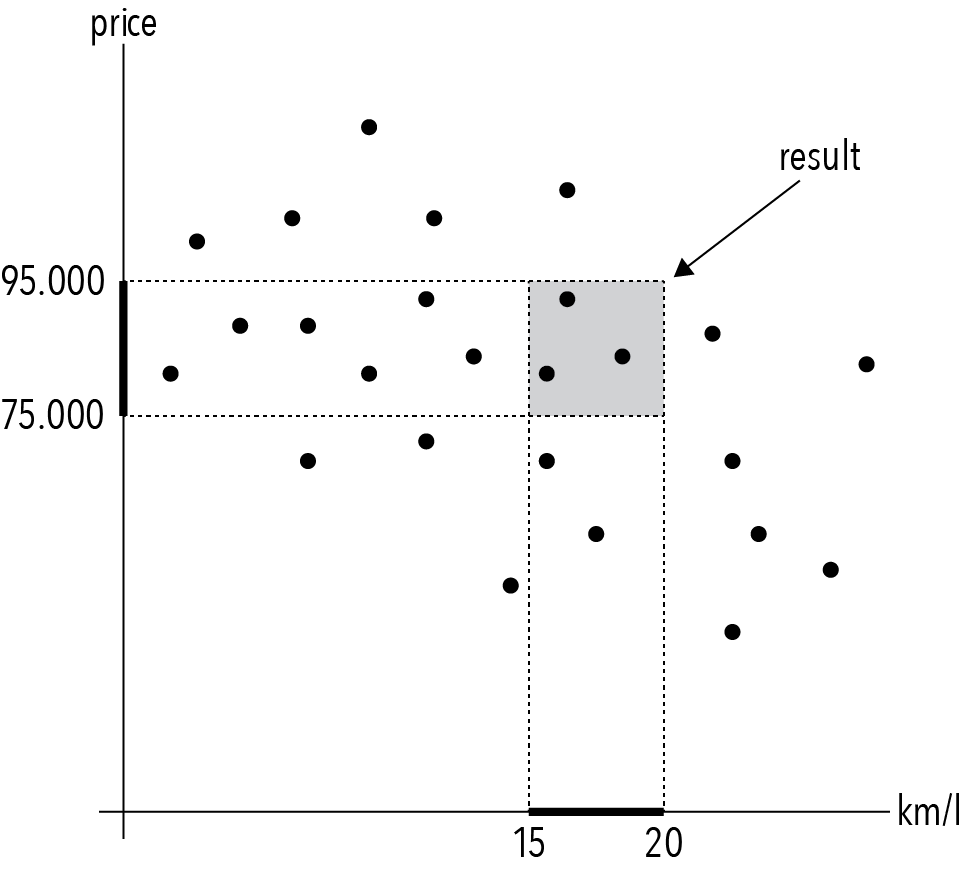
\includegraphics{pictures/introduction.png}
  \end{center}
\end{frame}

\begin{frame}{Preleminaries}
  \frametitle{Preleminaries}
  \begin{itemize}
    \item Alle koordinater er unikke
    \item Rank space
    \item $n$ er en potens af $2$
  \end{itemize}
\end{frame}

\begin{frame}{Orthogonal Range Searching}
  \frametitle{Orthogonal Range Searching}

  Vi er givet $n$ punkter fra $\mathbb{R}^2$ som vi ønsker at indsætte i en datastruktur sådan at vi kan svare effektivt på forespørgslen $q = [x_1, x_2] \times [y_1, y_2]$.
  Et punkt $p = (p_x, p_y)$ ligger i $q = [x_1, x_2] \times [y_1, y_2]$ hvis $p_x \in [x_1, x_2]$ og $p_y \in [y_1, y_2]$. Man kunne derfor sige at et 2-dimensionelt query består af to 1-dimensional sub-queries. Kommer til at virke for alle tre datastrukturer.
\end{frame}

\subsection{Previous data structures}

\begin{frame}{kd-træ}
  \frametitle{kd-træ}

  Givet $n$ punkter: Punkterne bliver sorteret efter $x$ eller $y$ på skift. Median bliver fundet og punkterne mindre end medianen bliver givet til venstre barn og punkterne højere end medianen bliver givet til højre barn. Et punkt per blad i træet.
  \begin{itemize}
    \item $\mathcal{O}(n)$ plads
    \item $\mathcal{O}(\sqrt{n} + k)$ tid
  \end{itemize}
\end{frame}

\begin{frame}{Opbygning}
  \frametitle{Opbygning af kd-træ}
  Det $\lceil \frac{n}{2} \rceil$'te element bliver valgt som median. Dette element fungerer som en skille-linje mellem de to punkt-mængder. Medianen bliver låst fast på denne plads i arrayet.
  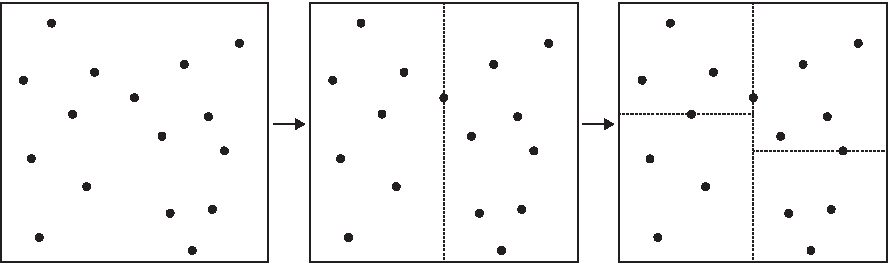
\includegraphics[scale=0.75]{pictures/kd_subdivision-eps-converted-to.pdf}
\end{frame}


\begin{frame}{Søgning}
  \frametitle{Søgning i kd-træ}
  \begin{center}
    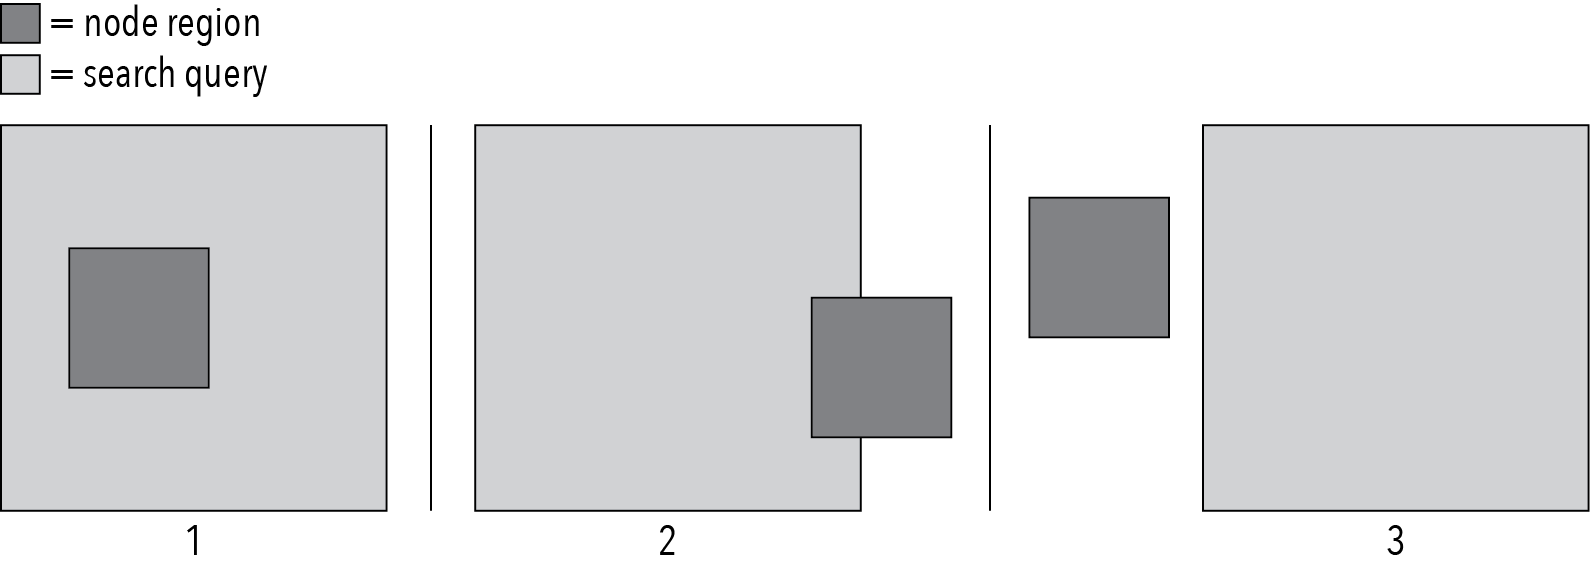
\includegraphics[scale=0.75]{pictures/search_query_overlap.png}
  \end{center}
\end{frame}


% Section and subsections will appear in the presentation overview
% and table of contents.

\section{Ball Inheritance Search}
\begin{frame}{BISintro}
  Ball Inheritance Search (BIS) er en datastruktur bygget som en simplificering af den datastruktur Chan et al laver.

\end{frame}


\subsection{Ball Inheritance Problem}

\begin{frame}{Ball Inheritance}

  \begin{itemize}
    \item Vi er givet et perfekt binært træ.
      \pause
    \item Roden indeholder $n$ punkter(bolde) som er blevet fordelt sådan at hvert blad lagrer et punkt. Elementerne i roden er sorteret.
      \pause
    \item Hver knude har en liste over hvilke bolder der går igennem den. De bolde ender så i træet med rod i den knude. Boldene i knudens liste har samme rækkefølge som boldene i forældre-knudens liste.
     \pause
    \item Løs: Givet en knude og et index i knudens liste, hvilket blad ender denne bold ved? Vi kan følge bolden 
     \pause
    \item Vi kan nu følge en bold fra en knude til et blad med $\mathcal{O}(\lg n)$ skridt.

  \end{itemize}
\end{frame}

\begin{frame}{Faster Queries}
  Vi ønsker at gøre antallet skridt fra en knude til et blad mindre. Vi udvider alfabetet på udvalgte niveauer.
  Det bruger
  \begin{itemize}
    \item $\mathcal{O}(\frac{n}{\epsilon}) = \mathcal{O}(n)$ plads
    \item $\mathcal{O}(\lg^\epsilon n)$ tid
  \end{itemize}
  hvor $\epsilon > 0$ er en arbitrær lille konstant. Space-time tradeoff.
  Vis koncept, tid og plads her
\end{frame}

\subsection{Ball Inheritance Search Data Structure}
\begin{frame}{Ball Inheritance Search}
  \begin{itemize}
    \item $\mathcal{O}(n)$ plads
    \item $\mathcal{O}(\lg n + k\cdot\lg^\epsilon n)$ tid, hvor $\epsilon > 0$ er en arbitrær lille konstant
  \end{itemize}
\end{frame}

\begin{frame}{x range}
  \frametitle{x-range}
  \begin{itemize}
    \item Vi oversætter vores query til rank space $[x_1, x_2] \times [y_1, y_2] \Rightarrow [\hat{x}_1, \hat{x}_2] \times [\hat{y}_1, \hat{y}_2]$.
      \pause

    \item Vi går ned til least common ancestor af $\hat{x}_1$ og $\hat{x}_2$ og herfra ned til $\hat{x}_1$ og $\hat{x}_2$. På den måde finder vi knuder der kun indeholder punkter i $[x_1, x_2]$.
  \end{itemize}
\end{frame}

\begin{frame}{y range}
  \frametitle{y-range}
  \begin{itemize}
    \item Vi har opdateret $[\hat{y}_1, \hat{y}_2]$ fra roden til både $\hat{x}_1$ og $\hat{x}_2$. Dvs vi ved hvilke bolde i hver knude vi fandt før der indeholder punkter i $[y_1, y_2]$.
      \pause
    \item  Vi har nu nogle knuder og lister over indeces i disse knuder. Det er præcis det problem ball inheritance løser. Vi kan nu bruge ball inheritance på alle disse knuder til at finde ud af hvilke blade der indeholder punkter i $[y_1, y_2]$.
  \end{itemize}
\end{frame}

\begin{frame}{ballinheritance}
  Vi har nu at hver knude der er fully contained laver ball inheritance på det y-range den får givet. Det tager $\mathcal{O}(k\cdot\lg^\epsilon n)$ tid. Det tager $\mathcal{O}(\lg n)$ at lave binær søgning og at gå fra roden til $\hat{x}_1$ og $\hat{x}_2$.
  \pause
  Det giver en kørselstid på $\mathcal{O}(\lg n + k\cdot\lg^\epsilon n)$ for at finde $k$ punkter.
\end{frame}

\begin{frame}{plads}
  Denne datastruktur bruger $\mathcal{O}(n)$ plads.
  \begin{itemize}
    \item Bit vectors.
      \pause
    \item Store hop (Kommer vi til)
      \pause
    \item Egentlig punkter
      \pause
    \item Binær søgning
  \end{itemize}
\end{frame}

\begin{frame}{Små hop}
  bla bla om pladsen og constant time query
\end{frame}

\begin{frame}{store hop}
  bla bla om pladsen
\end{frame}

\end{document}


